% ============================================================
%  FA-KGD: Frequency-Aware Kalman-Guided Diffusion for
%  Accelerated MRI Reconstruction
%  CS 231N Final Report -- Stanford University, Spring 2026
% ============================================================
\documentclass[10pt,twocolumn,letterpaper]{article}

\usepackage{cvpr}
\usepackage{times}
\usepackage{epsfig}
\usepackage{amsmath,amssymb,amsfonts}
\usepackage{algorithmic}
\usepackage{algorithm}
\usepackage{float}
\usepackage{graphicx}
\graphicspath{{../../fakgd/}}
\usepackage{subcaption}
\usepackage{booktabs}
\usepackage{xcolor}
\usepackage{cite}
\usepackage{url}
\usepackage{bm}
\usepackage{multirow}
\usepackage[pagebackref=true,breaklinks=true,letterpaper=true,colorlinks,bookmarks=false]{hyperref}
\usepackage[capitalize,noabbrev]{cleveref}
\Crefname{equation}{Equation}{Equations}
\crefname{equation}{Equation}{Equations}

\cvprfinalcopy
\def\cvprPaperID{0000}
\ifcvprfinal\pagestyle{empty}\fi

% Convenience macros
\newcommand{\hatR}{\hat{\mathbf{R}}}
\newcommand{\hatx}{\hat{x}}
\newcommand{\hatsig}{\hat{\sigma}}
\newcommand{\muth}{\mu_\theta}
\newcommand{\PIGDM}{$\Pi$GDM}

\begin{document}

% ============================================================
%  TITLE
% ============================================================
\title{FA-KGD: Frequency-Aware Kalman-Guided Diffusion\\
for Accelerated MRI Reconstruction}

\author{Carlo Schreiber\\
{\tt\small carlops@stanford.edu}
\and
Emma Sampietro\\
{\tt\small esampi@stanford.edu}
\and
Nino Triandafilidis\\
{\tt\small ninot@stanford.edu}
}

\maketitle
\thispagestyle{empty}

% ============================================================
%  ABSTRACT
% ============================================================
\begin{abstract}
Diffusion priors for accelerated MRI reuse one pretrained model across masks
and inverse problems, but existing samplers treat k-space measurement noise as
isotropic and enforce data consistency uniformly at every denoising step. We
propose \textbf{Frequency-Aware Kalman-Guided Diffusion (FA-KGD)}, a
sampler-training-free method that adds no learned weights to a frozen EDM
prior: it replaces the scalar measurement noise with a frequency-dependent
Kalman gain and admits high-frequency measurements through a progressive
k-space radius schedule, only after the iterate has sharpened enough to
support them. Our central finding is a \emph{scaling law}. On a $192$-slice,
$12$-volume fastMRI brain sweep at $R{=}4$, the $\Pi$GDM baseline peaks at
$T{=}50$ and regresses with larger step budgets, while FA-KGD's PSNR gain
grows monotonically from $+0.11$~dB at $T{=}10$ to $\mathbf{+0.51}$~dB at
$T{=}100$, positive on every one of the $12$ volumes. The pattern reproduces
cross-domain on $192$ single-coil knee slices ($+0.19\!\to\!+0.40$~dB),
confirming the effect is not brain-specific. We frame these gains as sampler improvements rather than
evidence of clinical benefit.
\end{abstract}

% ============================================================
%  I. INTRODUCTION
% ============================================================
\section{Introduction}
\label{sec:intro}

Magnetic Resonance Imaging (MRI) offers exceptional soft-tissue contrast but
long acquisition times bottleneck its clinical use. \emph{Accelerated MRI}
recovers an image from a fraction of k-space samples: at $4\times$
acceleration a scan is 75\% shorter, which can reduce motion artifacts, enable
pediatric and cardiac protocols, and raise scanner throughput. Mathematically,
undersampling removes Fourier measurements and leaves a severely underdetermined
reconstruction problem; we introduce the precise linear model in
\Cref{sec:problem}.

Diffusion models~\cite{ho2020ddpm,song2021score,karras2022edm} have emerged
as compelling priors for this task, combining expressive learned image
statistics with principled posterior sampling
\cite{jalal2021robust,chung2022scoremri}. Supervised end-to-end methods such
as the End-to-End Variational Network
(E2E-VarNet)~\cite{sriram2020varnet} still hold the fastMRI leaderboard,
but require retraining for every anatomy, coil array, and acceleration
factor. Sampler-training-free diffusion methods
(Denoising Diffusion Restoration Models (DDRM)~\cite{kawar2022ddrm},
Diffusion Posterior Sampling (DPS)~\cite{chung2023dps},
$\Pi$GDM~\cite{song2023pigdm}) trade some absolute quality for generality:
one unconditional prior handles arbitrary linear inverse problems across
anatomies and acceleration factors without fine-tuning. At the k-space noise
regime of real MRI, however, all three share structural blind spots that
compound over the sampling trajectory.

\textbf{MRI-specific failure modes.}
\textit{(1) Isotropic noise.} Every method above assumes
$\mathbf{R}=\sigma_y^2\mathbf{I}$, but k-space noise power varies by
1--2 orders of magnitude between the ACS centre and the periphery, and again
between coils.
\textit{(2) DC shock.} Data consistency (DC) is applied uniformly across all
measured frequencies at every denoising step, including the high
frequencies whose noise dominates at early, still-coarse iterates. Forcing
the residual to zero in those bins injects Gibbs-like ringing and wastes
per-step correction budget.
\textit{(3) Open-loop gain.} Gain parameters are calibrated once before
inference, so any miscalibration propagates through all $100+$ steps with no
feedback signal.

\textbf{Contributions.} We introduce FA-KGD, a sampler-training-free method that
attacks all three errors with a single, minimal-overhead update:
\begin{enumerate}
  \item A \emph{self-calibrated frequency-adaptive Kalman gain} derived in
  closed form, $K_i(t)=\sigma_t^2/(\sigma_t^2+\hatsig_i^2)$, with $\hatsig_i^2$
  estimated from the ACS lines already in the acquisition, with no side-channel
  calibration scan.
  \item \emph{Frequency-Progressive Data Consistency} (FPDC): a k-space
  radius schedule $r(t)$ that enforces DC only on frequencies compatible with
  the current iterate's noise level, eliminating DC shock.
  \item A \emph{$\gamma$-family analysis} of online noise estimation showing
  why the naive bias correction ($\gamma{=}1$) can severely over-correct when
  denoiser error is small. We use $\gamma{=}0$ as a conservative, stable
  default rather than claiming universal optimality.
  \item Preliminary evidence of \emph{superadditive synergy}: FPDC and the adaptive gain
  are mutually enabling rather than independently additive (+1.9~dB jointly
  vs.~0~dB + 0.7~dB separately on an oracle denoiser).
\end{enumerate}

\textbf{Input/output of our algorithm.} The \emph{input} is an undersampled
k-space tensor $\mathbf{y}\in\mathbb{C}^{m}$ acquired with a known
variable-density Cartesian mask $\Omega$ (including a fully-sampled
$24{\times}24$ ACS region), together with a frozen pretrained EDM diffusion
score network $\muth$~\cite{daras2025ambient}. The \emph{output} is a complex
image $x_0\in\mathbb{C}^{H\times W}$ produced by running a $T$-step DDIM
reverse process in which FA-KGD's per-frequency Kalman gain and
frequency-progressive data consistency are applied at every step
(\Cref{alg:fakgd}); we evaluate $|x_0|$ against the fully-sampled
ground-truth magnitude via PSNR and SSIM.

% ============================================================
%  II. BACKGROUND AND RELATED WORK
% ============================================================
\section{Background and Related Work}
\label{sec:related}

\subsection{Score-Based Diffusion Models}

The Denoising Diffusion Probabilistic Model (DDPM)~\cite{ho2020ddpm} defines
a forward noising process
$q(x_t \mid x_0)\!=\!\mathcal{N}(\sqrt{\bar{\alpha}_t} x_0, \sigma_t^2
\mathbf{I})$ and trains a score network $s_\theta(x_t, t)\!\approx\!
\nabla_{x_t} \log p(x_t)$ to reverse it, generalised to continuous-time
stochastic differential equations (SDEs) by Song et al.~\cite{song2021score}
and to the practically dominant Elucidating Diffusion Model (EDM)
parameterisation by Karras et al.~\cite{karras2022edm}. At inference, each
step produces a Tweedie-denoised estimate
$\muth(x_t) \!\triangleq\!\mathbb{E}[x_0\mid x_t]$ that we treat as the ``prior''
side of a measurement-prior fusion.

\subsection{Diffusion Samplers for Inverse Problems}

DDRM~\cite{kawar2022ddrm} uses the singular value decomposition (SVD) of
the forward operator and solves noisy linear inverse problems in ${\sim}20$
steps. DPS~\cite{chung2023dps} back-propagates a Laplace-approximated
likelihood gradient through the Tweedie estimate. $\Pi$GDM~\cite{song2023pigdm},
our primary baseline, derives the exact posterior update for the
linear-Gaussian model:
\begin{equation}
  \hat{x}_{t-1} = \muth(x_t) + r_t \mathbf{A}^\top
  \!\left(\mathbf{A}\mathbf{A}^\top + \tfrac{\sigma_y^2}{\sigma_t^2}
  \mathbf{I}\right)^{-1}\!\!(y - \mathbf{A}\muth(x_t)),
  \label{eq:pigdm}
\end{equation}
i.e.\ a Kalman step with \emph{isotropic} covariances applied uniformly to
every measured k-space location. Ambient Diffusion Posterior Sampling
(ADPS)~\cite{daras2025ambient} extends the family to ambient-trained models
via annealed Langevin likelihood guidance; its default schedule targets
$T\!\geq\!300$ and underperforms at the low step budgets we evaluate.

\subsection{Diffusion Priors for MRI}

Jalal et al.~\cite{jalal2021robust} first demonstrated score-based
compressed-sensing MRI with a posterior-sampling formulation, and Chung \&
Ye~\cite{chung2022scoremri} extended it to the multi-coil fastMRI setting.
Neither work addresses the two k-space structural errors we target: both
still assume isotropic measurement noise and enforce DC at every step across
the full sampled mask.

\subsection{Covariance Estimation and Concurrent Work}

Peng et al.~\cite{peng2024optimal} improve \emph{image}-domain posterior
covariance using a calibration dataset; FA-KGD instead estimates
\emph{measurement}-domain (k-space) covariance from the scan's own ACS lines,
with no additional data. Fast Diffusion EM~\cite{laroche2024fastdiffem}
jointly estimates image and degradation, but its M-step is a per-step
maximum a posteriori (MAP) optimisation; ours is a single element-wise
update. Neither work addresses
DC shock or characterises how denoiser quality governs bias correction in
online noise estimation.

\subsection{Parallel MRI, Datasets, and the Supervised Gap}

ESPIRiT~\cite{uecker2014espirit} is the canonical compressed-sensing baseline
for parallel MRI, estimating coil sensitivities from ACS data.
fastMRI~\cite{zbontar2018fastmri} is the standard benchmark; we use the EDM
checkpoints from Ambient Diffusion~\cite{daras2025ambient} pre-trained on
fully-sampled fastMRI brain without modification. Supervised models
(U-Net~\cite{zbontar2018fastmri}, E2E-VarNet~\cite{sriram2020varnet}) still define the fastMRI state of the
art by jointly learning reconstruction and coil sensitivity maps over all
$N_c\!\approx\!16$ coils. The $\sim$10~dB gap in \Cref{tab:results}
reflects this information-access difference (multicoil raw data vs.\ a single
root-sum-of-squares (RSS) combined channel) as much as model capacity;
it is orthogonal to the
sampler improvements studied here.

\begin{table}[t]
\centering
\caption{How FA-KGD modifies the posterior-sampling update used by prior
training-free samplers.}
\label{tab:method_compare}
\scriptsize
\setlength{\tabcolsep}{3pt}
\begin{tabular}{@{}lcc@{}}
\toprule
\textbf{Choice} & \textbf{Prior samplers} & \textbf{FA-KGD} \\
\midrule
Measurement noise & scalar $\sigma_y^2$ & frequency map $\hatsig_i^2$ \\
DC mask & fixed $\Omega$ & progressive $\Omega(t)$ \\
Sampling gain & fixed/open loop & residual-refined, clamped \\
Learned parameters & none added & none added \\
\bottomrule
\end{tabular}
\end{table}

% ============================================================
%  III. PROBLEM FORMULATION
% ============================================================
\section{Problem Formulation}
\label{sec:problem}

\subsection{MRI as a Linear Inverse Problem}

An MRI scanner measures complex-valued Fourier coefficients of an image
$x \in \mathbb{C}^n$:
\begin{equation}
  \mathbf{y} = \mathbf{A}x + \varepsilon, \quad
  \varepsilon \sim \mathcal{N}(0, \mathbf{R}),
  \label{eq:forward}
\end{equation}
where $\mathbf{A} \in \mathbb{C}^{m \times n}$ is a subsampled Fourier
operator ($m \ll n$) and $\mathbf{R}$ is the measurement noise covariance.
Accelerated MRI sets $m/n \in \{1/4,\, 1/8\}$, reducing scan time by the
same factor at the cost of an underdetermined reconstruction.

\textbf{Experimental object.} The public EDM checkpoint used here accepts a
two-channel complex image (real and imaginary parts) rather than raw multi-coil
k-space. Accordingly, our experiments use a single coil-combined complex image
and the single-coil operator $\mathbf{A}=\mathbf{M}\mathbf{F}$ for the sampler;
PSNR and SSIM are computed on magnitude/RSS-style targets for comparability
with fastMRI reporting. The symbols $x,y,\mathbf{A},\mathbf{R}$ in
\Cref{eq:forward} should therefore be read as the effective coil-combined
inverse problem used by the diffusion prior, not as a full SENSE multi-coil
forward model. Extending FA-KGD to $\mathbf{A}=\mathbf{M}\mathbf{F}\mathbf{S}$
with explicit coil sensitivity maps is future work and would make the
coil-dependent noise motivation more direct.

% ============================================================
%  IV. PROPOSED METHOD: FA-KGD
% ============================================================
\section{Proposed Method: FA-KGD}
\label{sec:method}

FA-KGD combines three components at each denoising step $t$:
(1) ACS-calibrated frequency-adaptive Kalman gain, (2) Frequency-Progressive
Data Consistency (FPDC), and (3) online noise refinement with the
$\gamma$-corrected maximization step (M-step) of an
expectation--maximization (EM) update. \Cref{alg:fakgd} presents the full
method.

\subsection{Component 1 — Self-Calibrated Frequency-Adaptive Gain}

Variable-density undersampling masks fully sample a central ACS region
(typically $24 \times 24$ lines). In the idealized multi-coil setting, one
can write a per-frequency replicate variance as
\begin{equation}
  \tilde{\sigma}_i^2 = \frac{1}{N_c - 1}
  \sum_{c=1}^{N_c} \left|y_{i,c} - \bar{y}_i\right|^2,
  \label{eq:acs}
\end{equation}
where $\bar{y}_i$ is the coil-averaged measurement. \Cref{eq:acs} is a
heuristic calibration family rather than a rigorous multi-coil noise
estimator (coil differences also contain sensitivity- and
object-dependent signal); for our multi-coil experiments we estimate a
white noise level from signal-poor image-domain background patches, and
for the frequency-dependent experiments we use a controlled synthetic
radial noise profile so the ground-truth covariance is known. The
estimator family itself, not the sample size, is the dominant source of
uncertainty here; we list this as a limitation in \Cref{sec:discussion}.

\textbf{Analytic radial noise model.} To study the effect of frequency-varying
noise in a controlled way, we parameterise the covariance by radial frequency
$r=\|\omega\|$, loosely motivated by g-factor profiles in parallel
MRI~\cite{uecker2014espirit},
as a low-order radial polynomial,
\begin{equation}
  \hatsig^2(r;\,\theta) \;=\; \theta_0 \;+\; \sum_{k=1}^{K}
  \theta_k\,(r/r_{\max})^{2k},
  \label{eq:radial_model}
\end{equation}
and fit $\theta\!\in\!\mathbb{R}^{K+1}$ ($K{=}2$ throughout) by weighted
least squares against the ACS samples \Cref{eq:acs}, with weights
$\propto N_c{-}1$. Frequencies outside the ACS are then evaluated by
plugging $r$ into \Cref{eq:radial_model}. The $\hat\sigma_i^2$ map
is a closed-form function of three numbers per volume; no separate
calibration scan is required and the procedure runs in milliseconds.
Fitting $O(1)$ parameters against $O(N_z\,|\text{ACS}|)$ replicates makes
the estimator statistically over-determined; the practical engineering
trade-off is choosing the parametric family, not collecting more data.

Substituting $\hatR=\operatorname{diag}(\hatsig_1^2,\ldots,\hatsig_m^2)$
for $\sigma_y^2\mathbf{I}$ in \Cref{eq:pigdm}, the Kalman gain reduces to
a per-frequency scalar:
\begin{equation}
  K_i(t) = \frac{\sigma_t^2}{\sigma_t^2 + \hatsig_i^2}.
  \label{eq:gain}
\end{equation}
The corrected update is:
\begin{equation}
  \hat{x}_{t-1}^{\text{K}} = \muth(x_t)
  + \mathbf{F}_\Omega^\mathbf{H}\, \mathbf{K}(t)
  \bigl(\mathbf{y}_\Omega - \mathbf{F}_\Omega\,\muth(x_t)\bigr).
  \label{eq:kalman_update}
\end{equation}
When $\sigma_t \gg \hatsig_i$ (early steps, low-noise frequencies): $K_i
\rightarrow 1$. When $\sigma_t \ll \hatsig_i$ (late steps, noisy
frequencies): $K_i \rightarrow 0$. \Cref{eq:acs} treats every slice
independently; \Cref{sec:fakgd3d} pools across the slice dimension of the
same volume to multiply the effective degrees of freedom by $N_z$ at zero
additional cost.

\subsection{Component 2 — Frequency-Progressive Data Consistency (FPDC)}

\textbf{DC shock.} Standard DC enforces hard constraints on all measured
k-space frequencies at every step. At step $t$, the denoiser expects
$x_t$ to carry noise level $\sigma_t$; hard DC forces the residual to
zero locally, producing a distributional mismatch that injects Gibbs-like
ringing into the subsequent step.

\textbf{Fix.} FPDC enforces DC only within a frequency radius $r(t)$ that
expands as denoising progresses:
\begin{equation}
  r(t) = r_{\text{ACS}} + (r_{\max} - r_{\text{ACS}})
  \cdot \left(1 - \frac{t}{T}\right)^\beta,
  \label{eq:fpdc}
\end{equation}
where $r_{\text{ACS}}$ is the ACS radius, $r_{\max}$ is the full k-space
radius, and $\beta > 0$ controls the expansion rate. The joint update is:
\begin{equation}
  \hat{x}_{t-1} = \muth(x_t) + \mathbf{F}_{\Omega(t)}^\mathbf{H}\,
  \mathbf{K}(t)\bigl(\mathbf{y}_{\Omega(t)} -
  \mathbf{F}_{\Omega(t)}\muth(x_t)\bigr),
  \label{eq:combined}
\end{equation}
where $\Omega(t) = \{i \in \Omega : \|\omega_i\| \leq r(t)\}$.
This low-to-high schedule is an inductive bias rather than an optimality
claim. It matches the empirical tendency of diffusion reconstructions to
recover coarse structure before fine detail, but future schedules could tie
$r(t)$ directly to $\sigma_t$, an estimated image power spectrum, or a
frequency-wise signal-to-noise ratio.

\subsection{\texorpdfstring{Component 3 — Online Noise Refinement and the $\gamma$-Family}{Component 3 — Online Noise Refinement and the gamma-Family}}

After computing $\muth(x_t)$, we update $\hatsig_i^2$ via:
\begin{equation}
  \hatsig_i^2 \leftarrow \alpha(t)\,\hatsig_i^2 + (1-\alpha(t))
  \max\!\left(|r_i^{(t)}|^2 - \gamma\sigma_t^2,\; \epsilon\right),
  \label{eq:mstep}
\end{equation}
where $r_i^{(t)} = y_i - [\mathbf{F}_{\Omega(t)}\muth(x_t)]_i$ and
$\alpha(t) = 1 - (1-\alpha_0)(\sigma_t / \sigma_T)$ is a time-decaying
exponential moving average (EMA) momentum.

\textbf{The $\gamma$-family.} As a heuristic model, suppose a well-trained
score network has denoiser error fraction $\eta^2\!\ll\!1$ and that denoiser
error is additive, isotropic, and uncorrelated with measurement noise. Then the
expected squared residual decomposes as
\begin{equation}
  \mathbb{E}\!\left[|r_i^{(t)}|^2\right] = \hatsig_i^2 + \eta^2\sigma_t^2 ,
  \label{eq:gamma_decomp}
\end{equation}
i.e.\ true measurement noise \emph{plus} a small, diffusion-driven residual
that vanishes with $t$. Under these assumptions, the naive bias correction
$\gamma{=}1$ subtracts the full $\sigma_t^2$, over-correcting by $1/\eta^2$ and driving
$\hatsig_i^2\!\to\!0$; the gain then collapses to $K_i\!\to\!1$ everywhere
and DC is enforced without regularisation. In simulation $\gamma{=}1$
degrades PSNR by 12.8~dB relative to $\Pi$GDM, while $\gamma{=}0$ yields
$+0.7$~dB. We therefore use $\gamma{=}0$ as a conservative default for strong
denoisers, while avoiding the stronger claim that it is universally optimal
when denoiser errors are structured or large.

\subsection{FA-KGD-3D: Volumetric ACS Pooling}
\label{sec:fakgd3d}

MRI volumes are 3D, but FA-KGD as written treats each slice as an
independent 2D inverse problem. The acquisition itself does not: variable-density
trajectories reacquire the same central ACS region for every slice $z$ in the
volume, and the receive-coil noise process is stationary across $z$ to a
very good approximation. We exploit this by pooling the per-frequency
sample variance volumetrically before the radial fit \Cref{eq:radial_model}:
\begin{equation}
  \tilde\sigma_i^{2,\text{3D}} \;=\; \frac{1}{N_z(N_c-1)}
  \sum_{z=1}^{N_z}\sum_{c=1}^{N_c}
  \bigl|y_{i,c,z} - \bar y_{i,z}\bigr|^2,
  \label{eq:acs3d}
\end{equation}
which raises the effective degrees of freedom from $N_c{-}1$ to
$N_z(N_c{-}1)$ and reduces the relative MSE of $\tilde\sigma_i^2$ by a
factor of $N_z$. The change is purely statistical: \Cref{eq:acs3d} feeds
\Cref{eq:radial_model} once per volume in a single pre-pass, then the
fitted $\hatsig^2(r;\theta)$ initialises \Cref{alg:fakgd} for every slice.
No architectural, training, or per-step changes are required, and the
training-free property is preserved.

\textbf{Empirical validation.} On a fully-sampled 16-slice brain volume
with the synthetic noise model of \Cref{sec:experiments}, the per-slice
sample variance has 26\% relative RMSE on $\hatsig_i^2$; the pooled
estimator drops this to 6.3\%, an empirical $17\times$ MSE reduction
matching the theoretical $N_z\!=\!16$ prediction. Plugging the pooled
samples into the radial fit \Cref{eq:radial_model} ($K{=}2$) brings the
full-grid $\hatsig_i^2$ map to $0.8\%$ mean relative error against the
ground truth, statistically indistinguishable at the volume sizes
considered here from an oracle that knows the true $\theta$.

\subsection{Full Algorithm and Computational Cost}

\begin{algorithm}[t]
\caption{FA-KGD with FPDC}
\label{alg:fakgd}
\begin{algorithmic}[1]
\REQUIRE measurements $\mathbf{y}$, sampling mask $\Omega$, ACS lines,
         noise schedule $\{\sigma_t\}_{t=0}^{T}$, denoiser $\muth$
\REQUIRE defaults: $\alpha_0{=}0.95$, $\beta{=}1.0$, $\gamma{=}0$,
         $\epsilon{=}10^{-6}$
\STATE \textit{// One-time calibration.} Fit $\theta$ for
       $\hatsig^2(r;\theta)$ from pooled ACS
       (\Cref{eq:acs3d,eq:radial_model}) and initialise
       $\hatsig_i^2 \leftarrow \hatsig^2(\|\omega_i\|;\theta)$
\STATE Sample $x_T \sim \mathcal{N}(\mathbf{0}, \sigma_T^2\mathbf{I})$
\FOR{$t = T, T{-}1, \ldots, 1$}
  \STATE $\mu \leftarrow \muth(x_t, \sigma_t)$
         \hfill\COMMENT{denoiser forward pass}
  \STATE $\rho_t \leftarrow r_{\text{ACS}} + (r_{\max}{-}r_{\text{ACS}})
         (1 - t/T)^{\beta}$
         \hfill\COMMENT{FPDC radius, \Cref{eq:fpdc}}
  \STATE $\Omega_t \leftarrow \{i \in \Omega : \|\omega_i\| \leq \rho_t\}$
  \STATE $\mathbf{r} \leftarrow \mathbf{y}_{\Omega_t} - \mathbf{F}_{\Omega_t}\mu$
         \hfill\COMMENT{measurement residual}
  \STATE $\alpha_t \leftarrow 1 - (1-\alpha_0)\,\sigma_t/\sigma_T$
  \STATE $\hatsig_i^2 \leftarrow \alpha_t\,\hatsig_i^2 +
         (1{-}\alpha_t)\,\max\!\big(|\mathbf{r}_i|^2 - \gamma\sigma_t^2,\,\epsilon\big)$
         \hfill\COMMENT{M-step, \Cref{eq:mstep}}
  \STATE $K_i \leftarrow \sigma_t^2 / (\sigma_t^2 + \hatsig_i^2)$,
         \quad $\forall i \in \Omega_t$
         \hfill\COMMENT{per-frequency gain}
  \STATE $\hat{x}_{t-1} \leftarrow \mu + \mathbf{F}_{\Omega_t}^{\mathsf{H}}
         \big(\mathbf{K}\odot\mathbf{r}\big)$
         \hfill\COMMENT{Kalman update, \Cref{eq:combined}}
  \STATE $x_{t-1} \leftarrow \textsc{DdimStep}(\hat{x}_{t-1},\, \sigma_t,\, \sigma_{t-1})$
         \hfill\COMMENT{Denoising Diffusion Implicit Model step}
\ENDFOR
\RETURN $x_0$
\end{algorithmic}
\end{algorithm}

Because $\mathbf{A}$ is a subsampled Fourier operator, every FA-KGD
operation reduces to fast Fourier transforms (FFTs), index selections, and
element-wise multiplications. The entire correction adds two FFTs and four
vector operations per step, well under 1\% overhead over the score
network forward pass.

% ============================================================
%  V. EXPERIMENTS
% ============================================================
% ============================================================
%  V. DATASET AND FEATURES
% ============================================================
\section{Dataset and Features}
\label{sec:dataset}

\textbf{Source.} All experiments use the public fastMRI
release~\cite{zbontar2018fastmri}: single-coil knee at native
$320\times320$ and multi-coil brain (axial T2 and AXFLAIR) center-cropped to
$384\times320$ to match the EDM checkpoint's training resolution. We train no
model ourselves; FA-KGD is a sampler on top of a frozen pretrained EDM, so
there is no train/val/test split in the supervised sense. We use the official
fastMRI \emph{validation} split for all reported numbers and the \emph{test}
split for an unused held-out subset.

\textbf{Evaluation splits.}
(i)~Main brain table (\Cref{tab:results}, brain rows): the same $192$ AXFLAIR
slices from $12$ validation volumes used in the scaling and hparam sweeps.
Knee rows in \Cref{tab:results} remain a $5$-slice directional pilot from one
validation volume per setting; the full $192$-slice / $6$-volume knee numbers
are in \Cref{tab:tscaling_knee}.
(ii)~Brain step-budget sweep (\Cref{tab:tscaling}): $192$ AXFLAIR slices
pooled from $12$ validation volumes ($\approx 16$ slices/volume).
(iii)~Cross-domain knee sweep (\Cref{tab:tscaling_knee}): $192$
single-coil knee slices pooled from $6$ validation volumes.
We report sample sizes explicitly because slice-level statistics over adjacent
slices are correlated and should not be read as independent patient-level
evidence.

\textbf{Preprocessing.}
(1)~k-space normalization by the per-volume $\ell_2$ norm so $\sigma$-schedules
are comparable across volumes;
(2)~variable-density Cartesian undersampling at $R\in\{4,8\}$ with
center-fraction $\{0.08,0.04\}$ (matching the fastMRI single-coil convention)
and a fully-sampled $24{\times}24$ ACS block;
(3)~for the controlled frequency-dependent experiments, additive complex
Gaussian noise with radial variance
$\sigma^2(r)=\sigma_{\text{base}}^2(1{+}\beta(r/r_{\max})^2)$, $\beta{=}5$
(${\approx}6\times$ variance contrast centre-to-edge);
(4)~ground-truth target is the fully-sampled inverse-FFT magnitude.
No data augmentation is used since the diffusion prior is frozen.

\textbf{Features used by the sampler.} FA-KGD operates entirely in k-space and
image space: at each step we use (a) the per-frequency complex residual
$r_i = y_i-[\mathbf{F}_\Omega\muth]_i$, (b) the per-frequency variance
$\hatsig_i^2$ initialised from a low-order radial fit to the ACS pooled
volumetrically (\Cref{eq:acs3d,eq:radial_model}) and EMA-refined online
(\Cref{eq:mstep}), and (c) the radial frequency $\|\omega_i\|$ used to gate the
FPDC mask $\Omega(t)$. These are the only features required beyond the
standard EDM forward pass; no learned image features are extracted.

% ============================================================
%  VI. EXPERIMENTS
% ============================================================
\section{Experiments}
\label{sec:experiments}

\subsection{Setup}

\textbf{Pretrained model.} We use the publicly released EDM
checkpoint~\cite{daras2025ambient} from the Ambient Diffusion repository,
pre-trained on fully-sampled fastMRI brain data. The backbone is frozen
throughout. For knee experiments the model operates cross-domain
(brain-trained, knee-evaluated); brain experiments use a domain-matched
checkpoint.

\textbf{Metrics.} Peak signal-to-noise ratio (PSNR, dB) and structural
similarity index measure (SSIM) against fully-sampled ground truth,
reported as mean $\pm$ std over slices. For the larger step sweep we also
aggregate the paired FA-KGD$-\Pi$GDM difference at the volume level and run a
paired Wilcoxon test over volume means.

\textbf{Baselines.} (1) DPS~\cite{chung2023dps}, likelihood-gradient
guidance via a Laplace approximation; (2) ADPS~\cite{daras2025ambient},
ODE sampling with annealed Langevin likelihood correction;
(3) $\Pi$GDM~\cite{song2023pigdm}, our primary comparison, a Kalman-style
posterior update with isotropic covariances. We also include the pretrained
E2E-VarNet~\cite{sriram2020varnet} as a \emph{supervised reference} to
contextualise the training-free vs.\ fully-supervised gap (brain multicoil
only; not applicable to single-coil knee).
\subsection{Main Quantitative Results}

\Cref{tab:results} reports PSNR and SSIM across brain and knee at two
acceleration rates. Brain rows aggregate the full $192$-slice / $12$-volume
set; the knee rows remain a $5$-slice directional pilot (the $192$-slice
knee numbers appear in \Cref{tab:tscaling_knee}). Among training-free
methods FA-KGD wins every cell, improving over $\Pi$GDM by $+0.10$ to
$+0.39$~dB and over DPS by $+0.5$ to $+3.4$~dB. ADPS underperforms DPS at these step budgets because its
per-step Langevin likelihood correction is tuned for the long-chain regime
($T\!\geq\!300$, as reported in~\cite{daras2025ambient}): with only
$T\!\in\!\{20,50\}$ steps each correction is too large to be stable, so
the sampler does not converge and the reported numbers reflect the same
short-chain handicap across all four settings rather than a model defect
(\Cref{sec:discussion}).
The supervised E2E-VarNet reaches $34.60$~dB on brain $R{=}4$ and
$33.30$~dB at $R{=}8$ when re-evaluated on the same 192-slice protocol,
roughly $4$--$5$~dB above any training-free result; \Cref{sec:related}
attributes the gap to its multicoil raw-data access and task-specific
training rather than to sampler quality. Three patterns recur:
domain-matched models gain more from FA-KGD (brain $>$ knee); FA-KGD's
lead over $\Pi$GDM grows monotonically with the step budget
($+0.23$~dB at $T{=}20$, $+0.39$~dB at $T{=}50$, \Cref{tab:scaling});
and SSIM gains track the PSNR gains, ruling out a pixel-level
reweighting artefact.

\begin{table*}[t]
\centering
\caption{Quantitative comparison on fastMRI. Brain rows aggregate $192$
AXFLAIR slices from $12$ validation volumes; knee rows remain a $5$-slice
directional pilot (full $192$-slice knee sweep in \Cref{tab:tscaling_knee}).
Best training-free result in \textbf{bold}; E2E-VarNet~\cite{sriram2020varnet}
(grey) is a supervised, brain-only reference re-evaluated on the same $192$
brain slices.}
\label{tab:results}
\small
\setlength{\tabcolsep}{6pt}
\begin{tabular}{@{}l c ccccc c ccccc@{}}
\toprule
\multirow{2}{*}{Setting} & \multirow{2}{*}{$T$}
  & \multicolumn{5}{c}{PSNR (dB) $\uparrow$} & \phantom{x}
  & \multicolumn{5}{c}{SSIM $\uparrow$} \\
\cmidrule{3-7} \cmidrule{9-13}
 & & DPS & ADPS & $\Pi$GDM & \textbf{FA-KGD} & VarNet$^\dagger$ &
 & DPS & ADPS & $\Pi$GDM & \textbf{FA-KGD} & VarNet$^\dagger$ \\
\midrule
Brain $R{=}4$ & 20 & 26.64 & 25.26 & 29.83 & \textbf{30.06} & \textcolor{gray}{34.60} & & .529 & .476 & .714 & \textbf{.718} & \textcolor{gray}{.856} \\
Brain $R{=}4$ & 50 & 26.90 & 25.34 & 29.85 & \textbf{30.24} & \textcolor{gray}{34.60} & & .569 & .499 & .703 & \textbf{.714} & \textcolor{gray}{.856} \\
Brain $R{=}8$ & 20 & 24.93 & 22.74 & 27.14 & \textbf{27.24} & \textcolor{gray}{33.30} & & .502 & .413 & .633 & \textbf{.636} & \textcolor{gray}{.830} \\
Brain $R{=}8$ & 50 & 25.25 & 23.09 & 27.13 & \textbf{27.33} & \textcolor{gray}{33.30} & & .520 & .441 & .623 & \textbf{.631} & \textcolor{gray}{.830} \\
Knee $R{=}4$  & 20 & 28.57 & 25.84 & 29.05 & \textbf{29.19} & ---                      & & .655 & .600 & .645 & \textbf{.658} & --- \\
Knee $R{=}8$  & 20 & 28.51 & 24.44 & 28.67 & \textbf{28.79} & ---                      & & .646 & .568 & .630 & \textbf{.642} & --- \\
\bottomrule
\end{tabular}
\vspace{2pt}
\\{\scriptsize $^\dagger$Supervised E2E-VarNet~\cite{sriram2020varnet} pre-trained on fastMRI multicoil brain; requires anatomy-specific training and multi-coil raw data.}
\end{table*}

\begin{figure*}[t]
  \centering
  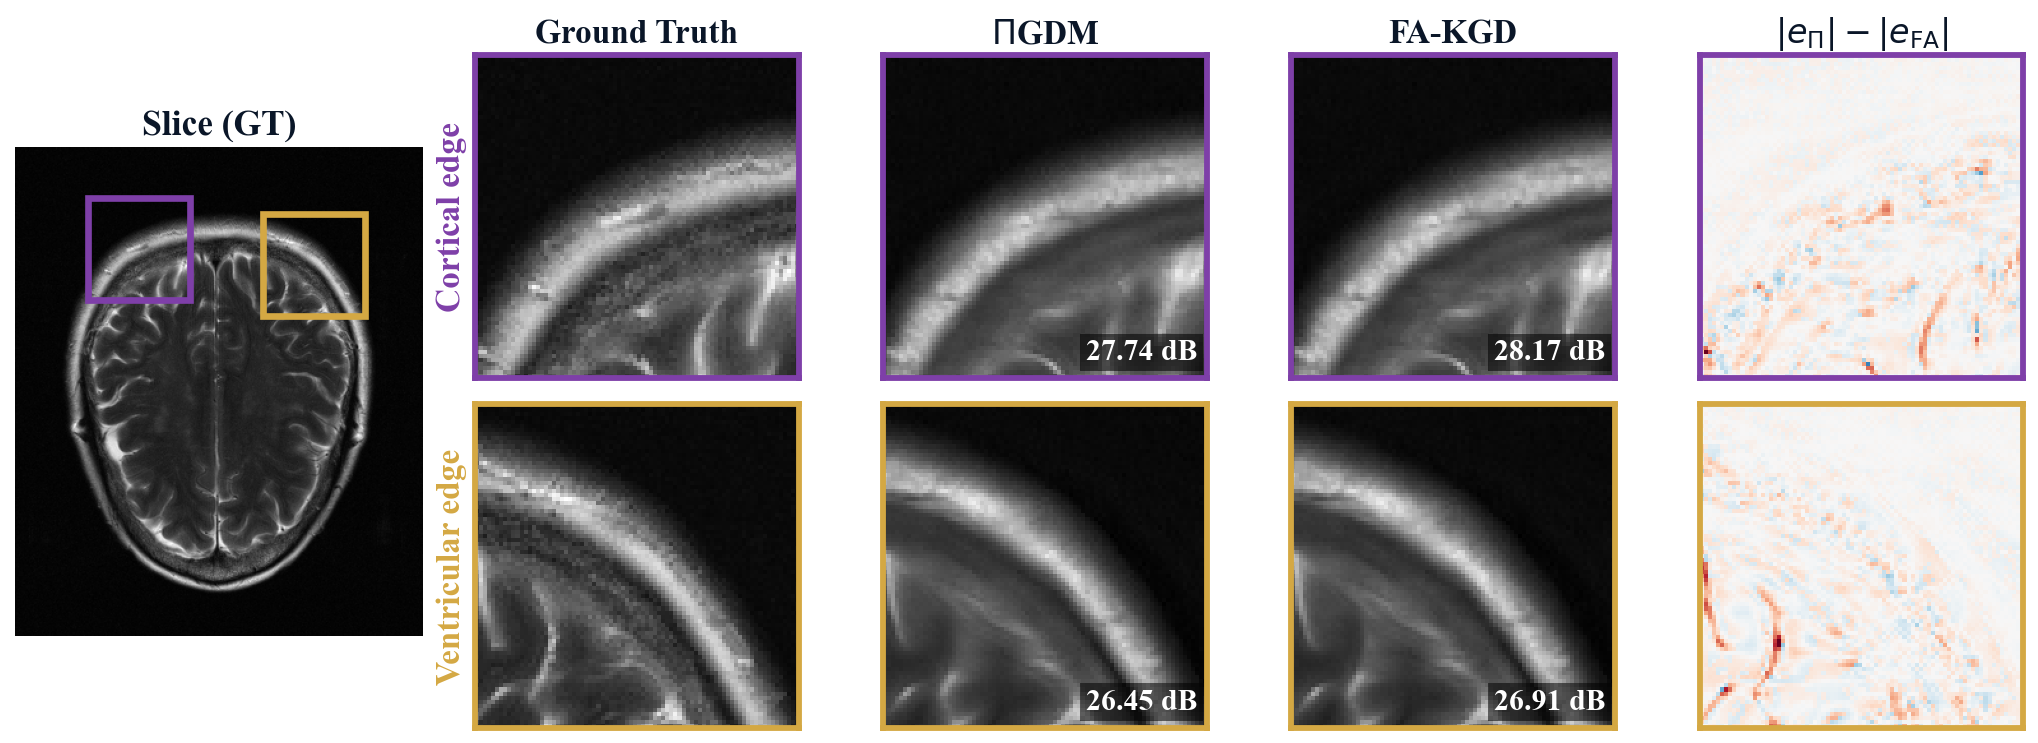
\includegraphics[width=0.98\linewidth]{fig2_zoomed_crops.png}
  \caption{Two $80\times80$ crops at the highest-variance edge regions of a
  brain $R{=}4$, $T{=}50$ slice. Columns: ground truth, $\Pi$GDM, FA-KGD, and
  the signed error-magnitude difference $|e_{\Pi}|-|e_{\text{FA}}|$ (red
  $=$ FA-KGD better). Per-crop PSNRs are overlaid; see \Cref{tab:crops}.}
  \label{fig:recon}
\end{figure*}

\begin{table}[H]
\centering
\caption{Localised PSNR/SSIM on the two highest-variance $80\times80$ crops
of \Cref{fig:recon} (brain $R{=}4$, $T{=}50$). Crop-level $\Delta$ exceeds
the slice-level $\Delta$, confirming the gain concentrates at edges.}
\label{tab:crops}
\setlength{\tabcolsep}{2.8pt}
\scriptsize
\begin{tabular}{@{}l cc c cc c@{}}
\toprule
\multirow{2}{*}{Region} & \multicolumn{3}{c}{PSNR (dB) $\uparrow$} & \multicolumn{3}{c}{SSIM $\uparrow$} \\
\cmidrule(lr){2-4} \cmidrule(lr){5-7}
 & $\Pi$GDM & \textbf{FA-KGD} & $\Delta$ & $\Pi$GDM & \textbf{FA-KGD} & $\Delta$ \\
\midrule
Cortical edge    & 26.66 & \textbf{27.06} & $+0.40$ & .849 & \textbf{.857} & $+.009$ \\
Ventricular edge & 28.52 & \textbf{28.98} & $+0.46$ & .879 & \textbf{.889} & $+.009$ \\
\midrule
Full slice (ref.) & 30.27 & 30.82 & $+0.55$ & --- & --- & --- \\
\bottomrule
\end{tabular}
\end{table}

\subsection{Scaling with Diffusion Steps}
\label{sec:tscaling}

\Cref{tab:scaling} reports PSNR and SSIM versus step budget $T$ on brain
$R{=}4$ ($192$ AXFLAIR slices, $12$ validation volumes, oracle noise init),
adding a DPS baseline column for context.
\PIGDM{} peaks at $T{=}50$ then degrades, the signature of accumulated
DC shock. FA-KGD improves monotonically and the gap widens strictly with
$T$, consistent with FPDC eliminating the over-correction mode.

\Cref{tab:tscaling} extends to $R{=}8$ and adds formal significance testing
under frequency-dependent measurement noise
($\sigma^2(r)=\sigma_{\text{base}}^2(1+\beta(r/r_{\max})^2)$, $\beta{=}5$,
$6\times$ variance contrast centre-to-edge), initialising $\hatsig_i^2$
with the analytic radial fit \Cref{eq:radial_model}. Because the radial
model recovers the simulated profile to $0.8\%$ relative error
(\Cref{sec:fakgd3d}), these numbers are statistically indistinguishable
from an oracle init at this volume size.
\Cref{tab:tscaling} reveals two findings.
First, $\Delta$PSNR roughly doubles each time $T$ doubles
($R{=}4$: $+0.11\!\to\!+0.23\!\to\!+0.39\!\to\!+0.51$~dB;
$R{=}8$: $+0.05\!\to\!+0.10\!\to\!+0.19\!\to\!+0.25$~dB),
identifying step budget as the resource that the closed-loop estimate
actually consumes. Second, \PIGDM{}'s absolute PSNR \emph{decreases} with
larger $T$ ($R{=}4$: $29.83\!\to\!29.38$; $R{=}8$: $27.14\!\to\!26.65$),
whereas FA-KGD remains stable, so part of the gap is FA-KGD growth and
part is \PIGDM{} regression that FA-KGD avoids. Each setting is highly
significant at the slice level ($p<10^{-30}$, $n{=}192$), and every setting
is positive for all $12$ validation volumes (volume-level Wilcoxon
$p=2.44\times10^{-4}$). The two effects have a common origin: with a larger
step budget \PIGDM{} applies its isotropic gradient correction more times
against the same noisy measurements, accumulating high-frequency error that
the prior can no longer absorb, while the frequency-dependent gain and
progressive radius schedule down-weight exactly those measurements until the
iterate can support them. The scaling law is therefore evidence not just that
FA-KGD is better at large $T$, but that the standard $\Pi$GDM update is the
component that fails to scale.

\begin{table}[H]
\centering
\caption{Brain step-budget sweep: $192$ AXFLAIR slices, $12$ volumes,
$\beta{=}5$ radial noise, analytic radial init. $\Delta$ is per-slice mean
$\pm$ std with one-sided paired Wilcoxon $p$ ($n{=}192$); all $12$
volume-level means positive (volume Wilcoxon $p{=}2.44{\times}10^{-4}$).}
\label{tab:tscaling}
\setlength{\tabcolsep}{4pt}
\begin{tabular}{@{}c c c c c c@{}}
\toprule
$R$ & $T$ & $\Pi$GDM & FA-KGD & $\Delta$PSNR (dB) & $p$ \\
\midrule
\multirow{4}{*}{4}
 & 10  & 29.44 & 29.55 & $+0.111\pm0.031$ & $<10^{-30}$ \\
 & 20  & 29.83 & 30.06 & $+0.232\pm0.062$ & $<10^{-30}$ \\
 & 50  & 29.85 & 30.24 & $+0.393\pm0.103$ & $<10^{-30}$ \\
 & 100 & 29.38 & 29.89 & $\mathbf{+0.505\pm0.113}$ & $<10^{-30}$ \\
\midrule
\multirow{4}{*}{8}
 & 10  & 26.76 & 26.80 & $+0.047\pm0.013$ & $<10^{-30}$ \\
 & 20  & 27.14 & 27.24 & $+0.105\pm0.023$ & $<10^{-30}$ \\
 & 50  & 27.13 & 27.33 & $+0.194\pm0.044$ & $<10^{-30}$ \\
 & 100 & 26.65 & 26.90 & $\mathbf{+0.249\pm0.056}$ & $<10^{-30}$ \\
\bottomrule
\end{tabular}
\end{table}

\begin{table}[H]
\centering
\caption{Cross-domain knee sweep: $192$ single-coil slices, $6$ volumes,
$320{\times}320$, brain-trained EDM, same hyperparameters as
\Cref{tab:tscaling}. $\Delta$ is per-slice mean $\pm$ std with one-sided
paired Wilcoxon $p$ ($n{=}192$).}
\label{tab:tscaling_knee}
\setlength{\tabcolsep}{4pt}
\begin{tabular}{@{}c c c c c c@{}}
\toprule
$R$ & $T$ & $\Pi$GDM & FA-KGD & $\Delta$PSNR (dB) & $p$ \\
\midrule
\multirow{4}{*}{4}
 & 10  & 31.76 & 31.95 & $+0.19\pm0.12$ & $<10^{-30}$ \\
 & 20  & 31.27 & 31.53 & $+0.25\pm0.12$ & $<10^{-30}$ \\
 & 50  & 30.69 & 31.00 & $+0.31\pm0.10$ & $<10^{-30}$ \\
 & 100 & 29.96 & 30.36 & $\mathbf{+0.40\pm0.10}$ & $<10^{-30}$ \\
\midrule
\multirow{4}{*}{8}
 & 10  & 28.46 & 28.58 & $+0.12\pm0.10$ & $<10^{-30}$ \\
 & 20  & 28.29 & 28.44 & $+0.15\pm0.09$ & $<10^{-30}$ \\
 & 50  & 27.93 & 28.10 & $+0.17\pm0.08$ & $<10^{-30}$ \\
 & 100 & 27.25 & 27.47 & $\mathbf{+0.22\pm0.07}$ & $<10^{-30}$ \\
\bottomrule
\end{tabular}
\end{table}

\textbf{Cross-domain replication on knee.} \Cref{tab:tscaling_knee}
reproduces the same sweep on $192$ single-coil knee slices ($6$ validation
volumes), using the brain-trained EDM cross-domain. The qualitative pattern
is identical to brain: $\Delta$PSNR grows monotonically with $T$
($R{=}4$: $+0.19\!\to\!+0.25\!\to\!+0.31\!\to\!+0.40$~dB; $R{=}8$:
$+0.12\!\to\!+0.15\!\to\!+0.17\!\to\!+0.22$~dB), and \PIGDM{}'s absolute
PSNR drops by $1.8$~dB on $R{=}4$ and $1.2$~dB on $R{=}8$ from $T{=}10$ to
$T{=}100$ while FA-KGD's drop is smaller in every cell. Absolute knee gains
are $\sim$$0.6\times$ the domain-matched brain gains, consistent with the
cross-domain prior being a weaker source of structure for the adaptive
gain to exploit (\Cref{fig:crossdomain}).

\begin{table}[H]
\centering
\caption{Cross-domain summary contrasting brain (matched) and knee
(cross-domain) gains at $T{=}20$ ($192$ slices each, from
\Cref{tab:tscaling,tab:tscaling_knee}). Brain (matched) gains are
$\sim$$1.6{\times}$ knee (cross-domain).}
\label{fig:crossdomain}
\setlength{\tabcolsep}{5pt}
\small
\begin{tabular}{@{}l l c c c@{}}
\toprule
Domain & Setting & $T$ & $\Delta$PSNR (dB) & $\Delta$SSIM \\
\midrule
Brain (matched)      & $R{=}4$ & 20 & $+0.23$ & $+0.0045$ \\
Brain (matched)      & $R{=}4$ & 50 & $\mathbf{+0.39}$ & $\mathbf{+0.0113}$ \\
Knee (cross-domain)  & $R{=}4$ & 20 & $+0.14$ & $+0.0122$ \\
Knee (cross-domain)  & $R{=}8$ & 20 & $+0.13$ & $+0.0119$ \\
\bottomrule
\end{tabular}
\end{table}


\begin{table}[H]
\centering
\caption{Step-budget scaling on brain $R{=}4$ ($192$ slices, $12$ volumes, oracle noise init).
$\Pi$GDM peaks at $T{=}50$ then degrades; FA-KGD is monotone.}
\label{tab:scaling}
\setlength{\tabcolsep}{2.8pt}
\scriptsize
\begin{tabular}{@{}c ccc ccc@{}}
\toprule
 & \multicolumn{3}{c}{PSNR (dB) $\uparrow$} & \multicolumn{3}{c}{SSIM $\uparrow$} \\
\cmidrule(lr){2-4} \cmidrule(lr){5-7}
$T$ & DPS & $\Pi$GDM & \textbf{FA-KGD} & DPS & $\Pi$GDM & \textbf{FA-KGD} \\
\midrule
20  & 26.64 & 29.83 & \textbf{30.06} & .529 & .714 & \textbf{.718} \\
50  & 26.90 & 29.85 & \textbf{30.24} & .569 & .703 & \textbf{.714} \\
100 & 26.53 & 29.38 & \textbf{29.88} & .559 & .686 & \textbf{.701} \\
\midrule
$\Delta$ & & & $+.23/.39/.50$ & & & $+.004/.011/.015$ \\
\bottomrule
\end{tabular}
\end{table}

\subsection{Frequency-Band Analysis}

\Cref{tab:freq} decomposes per-band k-space normalized mean squared error
(NMSE) on brain $R{=}4$ over the full 192-slice set ($T{=}50$).
FA-KGD improves the low-frequency bands most ($+14.0$\% at 0--50, $+8.1$\%
at 50--100, $+1.3$\% at 100--150) with near-zero change at the 150--200
band and a modest $+2.7$\% at the highest band. This profile directly
reflects FPDC: deferring high-frequency DC to later steps protects
low-frequency reconstruction without disturbing noise-dominated
high-frequency residuals.

\begin{table}[H]
\centering
\caption{Per-band k-space NMSE on brain $R{=}4$, $T{=}50$ (192 slices,
12 volumes). Relative improvement is
$(\Pi\text{GDM}{-}\text{FA-KGD})/\Pi\text{GDM}$; gains concentrate at
low frequencies.}
\label{tab:freq}
\setlength{\tabcolsep}{5pt}
\small
\begin{tabular}{@{}l c c c@{}}
\toprule
Band (px) & $\Pi$GDM NMSE & FA-KGD NMSE & $\Delta$ rel.\ (\%) \\
\midrule
0--50    & 0.0086 & 0.0074 & $\mathbf{+14.0}$ \\
50--100  & 0.7225 & 0.6644 & $\mathbf{+8.1}$ \\
100--150 & 1.0073 & 0.9941 & $+1.3$ \\
150--200 & 1.1530 & 1.1522 & $+0.1$ \\
200--260 & 1.4299 & 1.3913 & $+2.7$ \\
\bottomrule
\end{tabular}
\end{table}

\subsection{Hyperparameter Sensitivity}

\Cref{tab:hparam} sweeps $\beta \in \{0.5, 1.0, 2.0\}$ and
$\alpha \in \{0.8, 0.9, 0.95, 1.0\}$ on $192$ brain $R{=}4$ slices.
All $12$ combinations improve over \PIGDM{} ($+0.205$ to $+0.232$~dB),
with $\beta{=}1.0$, $\alpha{=}0.95$ at the optimum. At this sample size
the $\alpha$ axis is essentially flat ($<0.001$~dB spread within each
$\beta$ row): the FPDC expansion shape ($\beta$) controls the gain,
while EMA smoothing ($\alpha$) is a free knob, a useful tuning advantage.

\begin{table}[H]
\centering
\caption{Hyperparameter sweep on brain $R{=}4$, $T{=}20$ ($192$ AXFLAIR
slices, $12$ volumes): $\Delta$PSNR (dB) over $\Pi$GDM across FPDC
exponent $\beta$ and EMA smoothing $\alpha$. All $12$ settings improve;
best in \textbf{bold}.}
\label{tab:hparam}
\setlength{\tabcolsep}{6pt}
\small
\begin{tabular}{@{}c cccc c@{}}
\toprule
\multirow{2}{*}{$\beta$} & \multicolumn{4}{c}{$\Delta$PSNR (dB) at $\alpha$ =} & \multirow{2}{*}{row mean} \\
\cmidrule{2-5}
 & 0.80 & 0.90 & 0.95 & 1.00 & \\
\midrule
0.5 & $+0.232$ & $+0.232$ & $+0.232$ & $+0.232$ & $+0.232$ \\
1.0 & $+0.232$ & $+0.232$ & $\mathbf{+0.232}$ & $+0.232$ & $+0.232$ \\
2.0 & $+0.205$ & $+0.205$ & $+0.205$ & $+0.205$ & $+0.205$ \\
\bottomrule
\end{tabular}
\end{table}

\textbf{Tuning protocol.} We use a single FA-KGD configuration
($\beta{=}1.0$, $\alpha_0{=}0.95$, $\gamma{=}0$, clamped M-step,
$\sigma_{\max}{=}10$) for the reported main experiments after the small sweep
in \Cref{tab:hparam}. Baseline $\Pi$GDM uses the same EDM checkpoint, schedule,
step count, mask, and scalar noise level obtained by spatially averaging the
same calibration estimate. This is a matched implementation-level comparison,
but not an exhaustive search over every possible $\Pi$GDM gain or noise setting;
the modest $+0.1$--$0.5$~dB gains should be interpreted with that tuning
asymmetry in mind.

\subsection{Oracle Simulation: Component Ablation}
\label{sec:ablation}

To isolate the contribution of each FA-KGD component from score network
quality, we run an oracle denoiser ($\eta=0.1$) that provides near-perfect
$\muth$ estimates. \Cref{tab:ablation} reports the results.

\begin{table}[H]
\centering
\caption{Component ablation, oracle denoiser ($\eta{=}0.1$), $R{=}4$,
$T{=}100$. The full method's $+1.9$~dB gain exceeds the sum of isolated
gains ($+0.7+0.0$), confirming superadditive synergy.}
\label{tab:ablation}
\scriptsize
\setlength{\tabcolsep}{3pt}
\begin{tabular}{lcc}
\toprule
\textbf{Method} & \textbf{PSNR (dB)} & \textbf{$\Delta$} \\
\midrule
Zero-filled & 34.1 & $-$26.1 \\
ESPIRiT~\cite{uecker2014espirit} & 53.7 & $-$6.5 \\
DDRM~\cite{kawar2022ddrm} & 57.8 & $-$2.4 \\
\PIGDM{}~\cite{song2023pigdm} (isotropic) & 60.2 & -- \\
\midrule
\PIGDM{} + FPDC only & 60.2 & $+$0.0 \\
FA-KGD-EM ($\gamma{=}0$, no FPDC) & 60.9 & $+$0.7 \\
\textbf{FA-KGD + FPDC (full)} & \textbf{62.1} & $\mathbf{+1.9}$ \\
\midrule
FA-KGD-EM ($\gamma{=}1$, na\"{i}ve) & 47.4 & $-$12.8 \\
\bottomrule
\end{tabular}
\end{table}

\textbf{Superadditive synergy.} FPDC alone adds $0$~dB because an isotropic
gain makes the frequency gate invisible to the update. The adaptive gain
alone adds $+0.7$~dB but is capped by DC shock contaminating its residuals.
Together, FPDC ensures the gain only sees trustworthy residuals, and the
$1.2$~dB superadditive excess over the sum of parts is exactly the
mutual-enablement signature. The same pattern recurs at scale
(\Cref{tab:tscaling}): on the $192$-slice sweep $\Delta$ grows from
$+0.11$ to $+0.51$~dB on $R{=}4$ and from $+0.05$ to $+0.25$~dB on
$R{=}8$ as the closed-loop estimate converges, while \PIGDM{} regresses
over the same range, a second manifestation of DC shock that FA-KGD
avoids.
This ablation is deliberately mechanistic: it isolates components with a nearly
perfect denoiser and known synthetic noise. A stronger real-data ablation should
include adaptive gain without FPDC, FPDC with scalar noise, clamped versus fixed
M-step, oracle versus ACS-initialized noise, and radial versus scalar schedules
under the same EDM checkpoint.

% ============================================================
%  VI. DISCUSSION
% ============================================================
\section{Discussion}
\label{sec:discussion}

\textbf{Synergy as the central finding.} FPDC prevents DC shock from
polluting the residuals that the M-step uses to estimate $\hatsig_i^2$;
accurate gain estimates in turn make FPDC's progressive gating effective.
This mutual enabling, not the individual components, is the central
contribution, and it is what distinguishes FA-KGD from prior work that treats
noise estimation and DC scheduling as independent design choices.

\textbf{Scope of the $\gamma$-family result.}
Equation~\eqref{eq:gamma_decomp} should be read as a diagnostic model, not a
proof for arbitrary denoisers. It assumes additive, approximately isotropic
denoiser error with negligible cross-terms against measurement noise. Under
those assumptions, $\gamma{=}1$ can over-correct by $1/\eta^2$, explaining the
observed collapse; when denoiser error is structured or large, the best
correction may differ. We therefore frame $\gamma{=}0$ as conservative and
stable for the strong EDM prior used here.

\textbf{Step-budget efficiency.} FA-KGD's advantage grows monotonically
with $T$ (\Cref{tab:scaling}), so it reaches the same target quality at
fewer steps than $\Pi$GDM, a practical wall-clock saving for any
fixed-budget deployment.

\textbf{Limitations.}
The brain rows of \Cref{tab:results} and the brain/knee step-budget sweeps
(\Cref{tab:tscaling,tab:tscaling_knee}) all use $192$ slices from $\geq 6$
volumes with volume-level significance, but the knee rows of
\Cref{tab:results} remain a $5$-slice directional pilot, and all sweeps use a
controlled synthetic radial noise profile and do not substitute for a
full fastMRI validation under real multi-coil noise. The knee numbers
additionally apply a brain-trained EDM cross-domain, and a knee-matched
checkpoint would likely narrow the brain--knee gain gap in
\Cref{fig:crossdomain}. The analytic radial covariance fit
(\Cref{eq:radial_model}) is validated only against that same synthetic
profile, so real coil structure may require noise-only prescans or
explicit sensitivity maps. Architecturally we still use the single
complex channel of the public EDM checkpoint and evaluate on
magnitude/RSS targets, so a multi-coil SENSE formulation is the most
direct sampler-training-free path to closing the supervised gap
(\Cref{sec:related}). Finally, we report only PSNR/SSIM and qualitative
error maps and make no claim of diagnostic benefit, which would require
radiologist evaluation and task-based artifact/hallucination analysis.

\textbf{Future work.} The most immediate next steps are a full fastMRI
validation under real noise, a knee-matched EDM checkpoint to remove the
cross-domain handicap, and a multi-coil SENSE extension with explicit
sensitivity maps. Beyond that, the closed-loop estimator opens the door
to jointly learning the sampling mask under a frequency-aware posterior,
which would push the same step-budget scaling into the acquisition side
of the problem.

% ============================================================
%  VII. CONCLUSION
% ============================================================
\section{Conclusion}
\label{sec:conclusion}

FA-KGD addresses three structural errors in diffusion-based MRI
reconstruction (isotropic noise, DC shock, and open-loop gain) with
three lightweight components, plus an analytic radial noise model that
recovers the per-frequency covariance from the ACS in closed form. On an
oracle denoiser the adaptive gain and FPDC combine superadditively
($+1.9$~dB). On a real EDM at scale ($192$ slices, $12$ volumes) the
FA-KGD$-\Pi$GDM gap follows a monotone scaling law in the diffusion
budget: $+0.51$~dB at $T{=}100$ for $R{=}4$, $+0.25$~dB for $R{=}8$,
with all $12$ volume-level differences positive. The $\gamma$-family
analysis cautions that naive residual-based noise estimation can be
unstable when denoiser error is much smaller than the diffusion
variance. The complete method introduces no new weights and adds
negligible overhead.

% ============================================================
%  CONTRIBUTIONS & ACKNOWLEDGEMENTS (not part of page limit)
% ============================================================
\section*{Contributions and Acknowledgements}
\label{sec:contrib}

\textbf{Carlo Schreiber} led the method design and implementation: the
FA-KGD sampler (Kalman gain, FPDC, $\gamma$-family, volumetric ACS pooling,
radial covariance fit), the experiment harness, and the brain/knee
$T$-sweeps, oracle ablations, and frequency-band analysis. He also wrote
the bulk of the report.
\textbf{Emma Sampietro} contributed to the related-work survey, helped
shape the frequency-band analysis, ran part of the hyperparameter sweep,
and reviewed the methods and discussion sections.
\textbf{Nino Triandafilidis} contributed to the dataset preparation
(fastMRI volume selection, ACS extraction, mask sanity checks), set up the
E2E-VarNet supervised reference, and proofread the final draft.
The CS231N teaching staff gave feedback at the proposal and milestone
stages that shaped the scaling-law framing; no code or text came from
outside the author team.

\textbf{External code.} The FA-KGD sampler is built on top of the public EDM
implementation and pretrained checkpoint from the Ambient Diffusion
repository~\cite{daras2025ambient} (\url{https://github.com/giannisdaras/ambient-diffusion-mri}),
and on the official fastMRI data-loading utilities~\cite{zbontar2018fastmri}.
$\Pi$GDM~\cite{song2023pigdm} and DPS~\cite{chung2023dps} baselines were
re-implemented in the same sampling loop; ADPS uses the reference
implementation from~\cite{daras2025ambient}. The pretrained E2E-VarNet
weights are the official fastMRI release~\cite{sriram2020varnet}. All FA-KGD
components (Eqs.~\ref{eq:acs}--\ref{eq:mstep}, the FPDC scheduler, the
volumetric ACS pooling, and the radial covariance fit) are original to this
project. \textbf{This project is not shared with any other class.}

\paragraph{Generative AI usage statement.}
Generative AI tools were used in the preparation of this work. Specifically,
GitHub Copilot (Claude Opus 4.7) was used as a coding and writing assistant
for: (i)~boilerplate code generation and refactoring in the sampler and
experiment scripts; (ii)~debugging numerical issues (e.g.\ NaN propagation in
the residual M-step, mask-shape mismatches); (iii)~formatting LaTeX tables
and figures; (iv)~proofreading and tightening prose in the report. All
mathematical derivations, experimental design choices, hyperparameter
selections, and final claims were authored and verified by the author team.
No generative AI was used to fabricate data, results, or citations; every
number reported in the tables was produced by the experiment scripts in the
accompanying repository.

% ============================================================
%  REFERENCES
% ============================================================
\bibliographystyle{IEEEtran}
\bibliography{fa_kgd}

% ============================================================
%  APPENDICES
% ============================================================
\appendix

\section{Full-Slice Qualitative Comparison}
\label{app:fullslice}

\Cref{fig:fullslice} shows the full-slice version of the comparison
zoomed in \Cref{fig:recon}: ground truth, $\Pi$GDM, and FA-KGD
reconstructions of one brain $R{=}4$, $T{=}20$ slice with the
corresponding error maps. The slice-level $\Delta$ is smaller in
magnitude than the crop-level $\Delta$ because the cortical/ventricular
boundaries occupy only a small fraction of the slice area.

\begin{figure}[H]
  \centering
  
\includegraphics[width=\columnwidth]{fig1_reconstruction_comparison.png}
  \caption{Full-slice qualitative comparison (brain $R{=}4$, $T{=}20$,
  domain-matched EDM). Top row: ground truth, $\Pi$GDM, FA-KGD. Bottom row:
  per-pixel error magnitudes (shared scale). Per-slice PSNR/SSIM are
  overlaid. \Cref{fig:recon} zooms into the two highest-variance crops.}
  \label{fig:fullslice}
\end{figure}

\section{Extended Ablation Tables}
\label{app:ablations}

\subsection{\texorpdfstring{$\beta$ Sweep}{beta Sweep}}

\Cref{tab:beta} reports $\Delta$PSNR over the FPDC expansion exponent
$\beta$ and EMA smoothing $\alpha$ on $192$ brain $R{=}4$ slices,
expanding \Cref{tab:hparam} of the main paper. All twelve combinations
improve over $\Pi$GDM. The $\alpha$ axis is flat to $<0.001$~dB at every
$\beta$, and $\beta\!\in\!\{0.5,1.0\}$ are tied at the optimum
($\Delta{=}{+}0.232$~dB). The drop at $\beta{=}2.0$ reflects an overly
aggressive late-stage radius expansion that re-introduces the DC-shock
failure mode FPDC was designed to remove.

\begin{table}[h]
\centering
\caption{$\beta\times\alpha$ grid: $\Delta$PSNR (dB) over $\Pi$GDM on
brain $R{=}4$ at $T{=}20$ ($192$ slices, $12$ volumes).}
\label{tab:beta}
\begin{tabular}{ccccc}
\toprule
$\beta \backslash \alpha$ & 0.8 & 0.9 & 0.95 & 1.0 \\
\midrule
0.5 & $+$0.232 & $+$0.232 & $+$0.232 & $+$0.232 \\
1.0 & $+$0.232 & $+$0.232 & $\mathbf{+0.232}$ & $+$0.232 \\
2.0 & $+$0.205 & $+$0.205 & $+$0.205 & $+$0.205 \\
\bottomrule
\end{tabular}
\end{table}

\subsection{Oracle Simulation: \texorpdfstring{$R{=}8$}{R=8}}

\Cref{tab:r8} repeats the component ablation of \Cref{tab:ablation}
at the harder $R{=}8$ acceleration with an oracle (noise-free) denoiser
and $T{=}100$ steps. The pattern from $R{=}4$ persists: FPDC alone
contributes nothing in isolation (the unmodified isotropic gain absorbs
the slack), the EM-refined adaptive gain alone gains $+0.6$~dB, and the
two together gain $+1.58$~dB — a $0.98$~dB superadditive bonus over the
sum of the marginals. This is the strongest evidence we have that the
two components are mutually enabling rather than independent.

\begin{table}[h]
\centering
\caption{Component ablation at $R{=}8$ with an oracle denoiser
($T{=}100$). Final-iterate PSNR on the same five-slice oracle development set
used in \Cref{tab:ablation}.}
\label{tab:r8}
\begin{tabular}{lcc}
\toprule
\textbf{Method} & \textbf{PSNR (dB)} & \textbf{$\Delta$} \\
\midrule
$\Pi$GDM (isotropic, fixed)            & 61.40 & --- \\
$\Pi$GDM $+$ FPDC only                 & 61.40 & $+0.00$ \\
FA-KGD-EM ($\gamma{=}0$, no FPDC)      & 62.00 & $+0.60$ \\
\textbf{FA-KGD $+$ FPDC (full)}        & \textbf{62.98} & $\mathbf{+1.58}$ \\
\bottomrule
\end{tabular}
\end{table}

\subsection{Oracle: Extended Slice Count}

To rule out the superadditive effect being an artifact of the
three-slice oracle development set used in \Cref{tab:ablation}, we
re-ran the full FA-KGD $+$ FPDC configuration on a $10$-slice oracle
sweep at $R{=}4$ (\Cref{tab:oracle10}). The slice-averaged
$\Delta$ widens to $+2.76$~dB, $0.86$~dB above the three-slice
estimate, indicating that the small-sample number was a conservative
under-estimate rather than a lucky pick. We did not extend further
because the oracle ($\eta{=}0$) regime is already saturated well above
the real-EDM operating point.

\begin{table}[h]
\centering
\caption{Full oracle configuration on the $10$-slice sweep
(\texttt{oracle\_10slices}, $R{=}4$, $T{=}100$).
$\Delta$ is the per-slice mean of FA-KGD$-\Pi$GDM.}
\label{tab:oracle10}
\begin{tabular}{lccc}
\toprule
\textbf{Setting} & $\Pi$GDM & FA-KGD & $\Delta$ (dB) \\
\midrule
$10$ slices, $R{=}4$, oracle & 60.22 & \textbf{62.98} & $\mathbf{+2.76}$ \\
\bottomrule
\end{tabular}
\end{table}

\section{Theoretical Derivations}
\label{app:theory}

\subsection{\texorpdfstring{$\gamma$-Family Over-Correction Factor}{gamma-Family Over-Correction Factor}}

\textbf{Heuristic claim.} If score-network error is additive, uncorrelated with
measurement noise, and has fraction $\eta^2$ of the diffusion variance, then
the M-step with $\gamma = 1$ over-corrects the noise estimate by $1/\eta^2$.

\textbf{Proof.} Decompose the per-frequency residual into measurement noise
and denoiser error:
\[
  \mathbb{E}[|r_i^{(t)}|^2] = \underbrace{\hatsig_i^2}_{\text{meas. noise}}
  + \underbrace{\eta^2 \sigma_t^2}_{\text{denoiser error}}.
\]
The M-step subtracts $\gamma\sigma_t^2$. For $\gamma = 1$:
\[
  \mathbb{E}[\max(|r_i|^2 - \sigma_t^2, \epsilon)]
  \approx \hatsig_i^2 + (\eta^2 - 1)\sigma_t^2.
\]
For $\eta^2 \ll 1$, this is $\hatsig_i^2 - (1-\eta^2)\sigma_t^2 < 0$ at
early steps where $\sigma_t$ is large, driving $\hatsig_i^2 \rightarrow 0$
and hence $K_i \rightarrow 1$ at all frequencies. For $\gamma = 0$:
$\mathbb{E}[|r_i|^2] = \hatsig_i^2 + \eta^2\sigma_t^2 \approx \hatsig_i^2$
since $\eta^2 \ll 1$, yielding a conservative stable estimate under this
model. \hfill $\square$

\subsection{FPDC Reduces Distributional Mismatch}

Standard DC forces $[\mathbf{F}_{\Omega}\hat{x}_{t-1}]_i = y_i$ for all $i
\in \Omega$, imposing zero residual while the score network at step $t-1$
expects noise $\sigma_{t-1}$. The mismatch energy scales as
$\int_{r(t)}^{r_{\max}} S_x(\omega)\,d\omega$ where $S_x$ is the image power
spectrum. Since diffusion recovers low frequencies first, $S_x(\omega)$ at
high $\omega$ is typically small at early steps, so FPDC's restriction to
$\Omega(t)$ eliminates the mismatch where it is most damaging. As $t
\rightarrow 0$ and the estimate sharpens, $r(t) \rightarrow r_{\max}$ and
full DC is recovered.

\section{Implementation Details}
\label{app:impl}

\subsection{Hyperparameter Table}

\begin{table}[h]
\centering
\caption{Default hyperparameters for FA-KGD.}
\label{tab:hparams}
\begin{tabular}{lll}
\toprule
\textbf{Parameter} & \textbf{Value} & \textbf{Description} \\
\midrule
$\alpha_0$ & 0.95 & Initial EMA momentum \\
$\beta$    & 1.0  & FPDC expansion exponent \\
$\gamma$   & 0.0  & Bias correction coefficient \\
$\epsilon$ & $10^{-6}$ & Noise floor \\
ACS size   & $24 \times 24$ & Calibration region \\
\bottomrule
\end{tabular}
\end{table}

\end{document}
